\documentclass{article}
\usepackage{amsmath,amssymb}
\usepackage{tikz}
\usepackage{enumitem}
\usepackage{geometry}
\geometry{margin=1in}

\title{Peer-graded Assignment: Trees assignment}
\date{}
\begin{document}

\maketitle

\section*{Question 1}

Consider the following multigraph \( G \) with vertices \( x, y, z, w \), where two edges exist between \( w \) and \( z \):

\begin{center}
\begin{tikzpicture}[scale=1.3, every node/.style={circle, fill=black, inner sep=1.5pt}]
  \node[label=above:\(x\)] (x) at (0,2) {};
  \node[label=right:\(y\)] (y) at (2,0) {};
  \node[label=below:\(z\)] (z) at (0,-2) {};
  \node[label=left:\(w\)] (w) at (-2,0) {};

  \draw (x) -- (y);
  \draw (x) -- (w);
  \draw (y) -- (w);
  \draw (y) -- (z);
  \draw (w) .. controls (-2.5,-1.2) .. (z);
  \draw (w) .. controls (-1.5,-1.0) .. (z); % second edge (w,z)
\end{tikzpicture}
\end{center}

\begin{enumerate}[label=\arabic*.]
  \item \textbf{Degree sequence of \( G \):}
  \[
  \deg(x) = 2, \quad \deg(y) = 3, \quad \deg(z) = \mathbf{3}, \quad \deg(w) = \mathbf{4}
  \]
  Therefore, the degree sequence is:
  \[
  (4, 3, 3, 2)
  \]

  \item \textbf{Draw two non-isomorphic spanning trees of \( G \):}

  \begin{center}
  \begin{tikzpicture}[scale=1.1, every node/.style={circle, draw, inner sep=1pt}]
    \node[label=above:\(x\)] (x) at (0,2) {};
    \node[label=right:\(y\)] (y) at (2,0) {};
    \node[label=below:\(z\)] (z) at (0,-2) {};
    \node[label=left:\(w\)] (w) at (-2,0) {};
    \draw[thick] (x) -- (y);
    \draw[thick] (y) -- (w);
    \draw[thick] (y) -- (z);
  \end{tikzpicture}
  \quad\quad
  \begin{tikzpicture}[scale=1.1, every node/.style={circle, draw, inner sep=1pt}]
    \node[label=above:\(x\)] (x) at (0,2) {};
    \node[label=right:\(y\)] (y) at (2,0) {};
    \node[label=below:\(z\)] (z) at (0,-2) {};
    \node[label=left:\(w\)] (w) at (-2,0) {};
    \draw[thick] (x) -- (w);
    \draw[thick] (w) -- (z);
    \draw[thick] (z) -- (y);
  \end{tikzpicture}
  \end{center}

  \item \textbf{Adjacency matrix \( A \) of \( G \):}  
  Vertex order: \( (x, y, z, w) \)
  \[
  A =
  \begin{bmatrix}
    0 & 1 & 0 & 1 \\
    1 & 0 & 1 & 1 \\
    0 & 1 & 0 & 2 \\
    1 & 1 & 2 & 0 \\
  \end{bmatrix}
  \]

  \item \textbf{What does the sum of elements in \( A \) tell you about \( G \)?} \\
  The sum of all elements in \( A \) is:
  \[
  1+1+1+1+1+1+2+2 = 14
  \]
  Since each edge is counted twice in the adjacency matrix of an undirected graph, the number of edges is:
  \[
  \frac{14}{2} = 7
  \]
  Therefore, \( G \) has 7 edges.
\end{enumerate}

\newpage

\section*{Question 2}

\begin{enumerate}[label=\arabic*.]
  \item \textbf{Draw a binary search tree to store 14 records:}

  A balanced BST of 14 nodes can be built with root at 7 to minimize depth.

  \begin{center}
  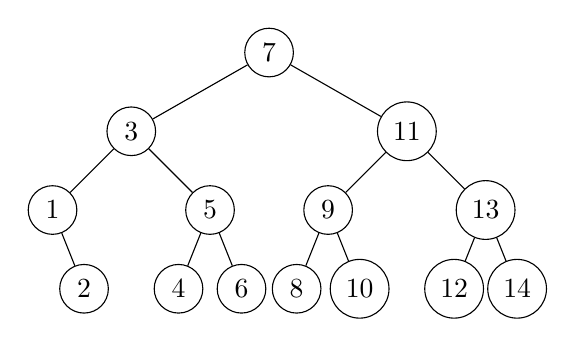
\begin{tikzpicture}[level distance=10mm,
    every node/.style={circle, draw, minimum size=6mm},
    level 1/.style={sibling distance=35mm},
    level 2/.style={sibling distance=20mm},
    level 3/.style={sibling distance=8mm}
    ]
    \node {7}
      child {node {3}
        child {node {1}
          child[missing]
          child {node {2}}}
        child {node {5}
          child {node {4}}
          child {node {6}}}
      }
      child {node {11}
        child {node {9}
          child {node {8}}
          child {node {10}}}
        child {node {13}
          child {node {12}}
          child {node {14}}}
      };
  \end{tikzpicture}
  \end{center}

  \item \textbf{Maximum number of comparisons to find any existing record:}

  The maximum number of comparisons equals the height of the tree:
  \[
  \lceil \log_2(14 + 1) \rceil = \lceil \log_2(15) \rceil = \lceil 3.9 \rceil = 4
  \]
  So the maximum number of comparisons required is:
  \[
  \boxed{4}
  \]
\end{enumerate}

\end{document}
